%% There is extensive work in the area of symbolic execution and automated testing.  In this chapter, we review the use of symbolic execution on commodity software for automated test case generation (Section~\ref{sec:relwork:atcg}), with an emphasis on how previous work addresses the environment problem (Section~\ref{sec:relwork:envproblem}).  We specifically review the work on parallelizing symbolic execution (Section~\ref{sec:relwork:parsymbex}), and discuss existing approaches related to symbolic tests (Section~\ref{sec:relwork:symtests}).


In this chapter, we review the existing work that touches on the environment problem in symbolic execution.
%
We start with a brief overview of the most important symbolic execution engines that advanced the state of the art and made the technique applicable to real-world software (Section~\ref{sec:relwork:atcg}).
%
We then systematize the approaches these tools took to address the environment problem (Section~\ref{sec:relwork:envproblem}).
%
The last part of the chapter covers the use of symbolic execution for high-level languages, which is a particular focus of our work (Section~\ref{sec:relwork:interplang}).


%%%%%%%%%%%%%%%%%%%%%%%%%%%%%%%%%%%%%%%%%%%%%%%%%%%%%%%%%%%%%%%%%%%%%%%%%%%%%%%%

\section{Symbolic Execution for Real-world Software Testing: A Brief History}
\label{sec:relwork:atcg}

%% King~\cite{king:symbolic:2} described symbolic execution as a practical middle ground between testing a program with a set of concrete inputs and using formal correctness proofs.  The paper introduced EFFIGY, an interactive symbolic execution tool where developers manually step through paths and switch states in the execution tree.  However, the tool could only handle small programs written in a custom language supporting basic integer operations, and had limited performance, due to limited solver capabilities.

Symbolic execution was introduced almost four decades ago as a test case generation technique~\cite{king:symbolic:2, boyer:symbolic}.  The first tools worked on domain-specific languages, supported basic numeric operations, and were mostly used for interactive debugging.  The effectiveness of the technique on more complex programs was limited by the lack of efficient and expressive constraint solvers and by slow hardware.

%% It was only in the past decade that symbolic execution has become a feasible approach to test generation for real-world software, with the advent of modern constraint solvers, such as Chaff~\cite{chaff}, MiniSAT~\cite{minisat}, STP~\cite{stp}, Z3~\cite{Z3}, or CVC~\cite{cvc}, and the exponential increase in hardware performance.  Our tools build on this foundation, too---both Cloud9 and Chef resort to the STP solver for all symbolic queries, such as branch feasibility checks.

The exponential increase in hardware performance and the availability of fast off-the-shelf constraint solvers~\cite{chaff,minisat,stp,Z3,cvc} amplified the research in symbolic execution.  Over the past decade, the new generation of symbolic execution engines produced test suites and found bugs on real-world software, ranging from small system utilities to large application suites.

In this section, we highlight the most important tools and discuss the techniques that expanded the applicability of symbolic execution on real-world software.  Whenever appropriate, we touch on the environment problem; however, we cover it extensively later on, in Section~\ref{sec:relwork:envproblem}.

\paragraph{Concrete + Symbolic Execution}

To support real-world programs, a symbolic execution engine must be prepared to deal with all language features and calls into the environment.
%
A first solution introduced by early engines, such as DART~\cite{dart} and CUTE~\cite{cute}, is to execute the program normally, using concrete inputs, while maintaining the symbolic execution state in the areas of interest.
%
When the symbolic semantics are not available, such as inside external library calls, the program execution would still be able proceed.
%
By using this approach, these tools found crashes in small-to-moderate C programs, such as protocol implementations and data structure libraries.

This form of execution is also called concolic (\emph{conc}rete + symb\emph{olic}), or ``whitebox fuzzing''.  The symbolic execution space is explored through successive runs of the program with concrete inputs.  The symbolic constraints collected at each run are used to generate new inputs, which are used in subsequent executions.


\paragraph{Specialized Solver Support}

%% In addition, real-world software generates constraints that are hard to reason about, containing expressions such as memory accesses from symbolic addresses, or complex arithmetic operations such as bit-wise multiplication and division.  Without solver support, a symbolic execution engine ends up concretizing the state or abandoning the path, hence losing completeness.

While the concolic approach helps engines avoid stumbling upon unsupported parts of the execution, it does not solve the problem of providing symbolic semantics for the target program.
%
In particular, a major limitation of the early symbolic execution engines was the lack of support for reasoning precisely and efficiently about common expressions involving binary arithmetic and memory access.  For instance, DART and CUTE used a solver only for linear integer constraints, which limited the scope of the symbolic analysis.

Subsequent symbolic execution engines took advantage of new breakthroughs in constraint solving and employed high-performance off-the-shelf solvers, such as Z3~\cite{Z3}, STP~\cite{stp}, or CVC~\cite{cvc}.  These solvers can reason efficiently about a large set of operations commonly encountered in program execution.
%
For example, the EXE~\cite{exe} symbolic execution engine was among the first to employ such a solver (STP), which was co-designed with EXE to accurately express machine operations in low-level languages such as C.
%
EXE modeled the program memory as a flat array of bytes, with support for arbitrary pointer reads and writes, mixed with fixed-width integer operations.
%
As a result, EXE targeted and found bugs in larger system software such as the \codebit{udhcpd} DHPC server, packet filters, and the \codebit{pcre} Perl regular expression library.

\paragraph{Low-level Symbolic Interpretation}

DART, CUTE, and EXE implemented symbolic execution at the C source code level, by using CIL~\cite{cil} to instrument the code with additional statements that maintain the symbolic state as the program executes.
%
However, this approach is tedious.  Even for a low-level language like C, the size of the language specification is about 200 pages\footnote{This figure refers to the C99 standard ISO/IEC 9899:1990 -- {\urlstyle{same}\url{http://www.iso.org/iso/iso_catalogue/catalogue_ics/catalogue_detail_ics.htm?csnumber=17782}}.}, so supporting all language features symbolically is an extensive engineering effort.  Moreover, the engineering cost would increase for more complex languages, such as C++.

%% Instead, the current state-of-the-art symbolic execution engines target lower-level compiled representations of programs, , which consist of a smaller set of simpler instructions, with an extensive and stable specification.

Instead, the current state-of-the-art symbolic execution engines take advantage of the fact that C, C++, and other languages are compiled to a lower-level representation, such as x86 binary or LLVM~\cite{llvm} bytecode, which is simpler to reason about~\cite{godefroid:fuzz,klee,bitBlaze,s2eSystem,mayhem}.  Two prominent examples are SAGE and KLEE.

SAGE~\cite{sage2012,godefroid:fuzz}---the best known use of symbolic execution in production---performs concolic execution at binary level.
%
This enables SAGE to target large applications with deep execution paths, such as Windows format parsers and Microsoft Office applications.
%
SAGE found thousands of Windows vulnerabilities at development time.

%% To target systems of increasing complexity, symbolic execution engines needed to address the environment problem.
%% %
%% KLEE~\cite{klee} was the first symbolic execution engine to target system software that communicates with its environment.  KLEE provides robust support for complex system software by having the software compiled to LLVM~\cite{llvm} IR, which is then interpreted symbolically.
%% %
%% KLEE~\cite{klee} introduced environment models as approximations of the real OS interface: the models replace parts of the standard C library and provided support for files.
%% %
%% This resulted in KLEE uncovering crashes and generating test suites with over 90\% coverage on average in the popular Coreutils utilities (e.g., \codebit{ls}, \codebit{echo}), testing Busybox and an OS kernel.
%% %
%% Our Cloud9 system builds on top of KLEE, providing symbolic primitives for a large fraction of the POSIX interface, as well as adding support for parallel symbolic execution.

KLEE~\cite{klee} is arguably the most popular symbolic execution engine, having served as a foundation for a wide range of other tools.
%
KLEE works as a symbolic interpreter for LLVM IR bytecode, obtained by compiling source programs using an LLVM-based compiler such as Clang.
%
KLEE was designed to target systems code, such as command line utilities (e.g., the popular \codebit{ls} or \codebit{echo}).  Since these systems call into the operating system, which is not available as LLVM IR, KLEE employs \emph{models} that approximate the real OS interface.
%
The KLEE models replaced parts of the standard C library and were linked with the target program, providing basic support for file operations---the most common dependency among the targeted utilities.
%
Unmodeled system calls were still allowed, by passing them to the host environment, executed concretely on behalf of the KLEE process.
%
KLEE found bugs and generated test suites with over 90\% statement coverage on average in the Coreutils suite.  It also found bugs in other systems software, such as Busybox and the HiStar kernel.

\paragraph{``In-vivo'' Symbolic Execution}

Targeting low-level representations, such as x86, has an additional advantage: it blurs the line between the program and its environment.  A program, its libraries, and the entire operating system, all execute the same CPU instruction set, which would be targeted by the symbolic execution engine.
%
This approach is particularly convenient when the target program is deeply integrated in the system, such that there is no clear separation between the program and its environment.

Full-VM symbolic execution engines, such as S2E~\cite{s2eSystem} and BitBlaze~\cite{bitBlaze}, leverage this approach in order to run symbolically any part of the software stack ``in-vivo'', without the need of the program source code, nor operating system models.
%
The program state effectively is the CPU state (registers, flags, etc.) and the contents of the physical memory.
%
I/O would still need to be modeled, as it constitutes the CPU environment; for instance, S2E provides symbolic models for devices, when testing their drivers running in a kernel.
%
Most notably, S2E discovered vulnerabilities in several Windows device drivers, some of whom were Microsoft-certified~\cite{ddt}.

Symbolic execution also found use in security testing~\cite{aeg,mayhem,bitBlaze}.  For this task, reaching vulnerabilities is more important than achieving completeness, so engines in this space resort to simplifications to increase performance and reach deeper executions in larger programs, at the expense of losing completeness.
%
For example, the AEG~\cite{aeg} tool uses symbolic analysis to both find bugs and automatically generate exploits (get a shell) from the bugs.  AEG uses heuristics that prioritize buggy paths and employs simple operating system models that minimize path explosion.
%
The Mayhem~\cite{mayhem} tool employs a simplified symbolic memory model where write addresses are concretized.
%
Both tools found exploitable vulnerabilities in Linux and Windows programs.

%% Handling real-world targets: C, C++ (KLOVER), parallel systems (explain the two ways to run these systems symbolically, depending on what bugs we're looking for).


%%%%%%%%%%%%%%%%%%%%%%%%%%%%%%%%%%%%%%%%%%%%%%%%%%%%%%%%%%%%%%%%%%%%%%%%%%%%%%%%

\section{Tackling the Environment Problem in Symbolic Execution}
\label{sec:relwork:envproblem}

\begin{figure}
  \centering
  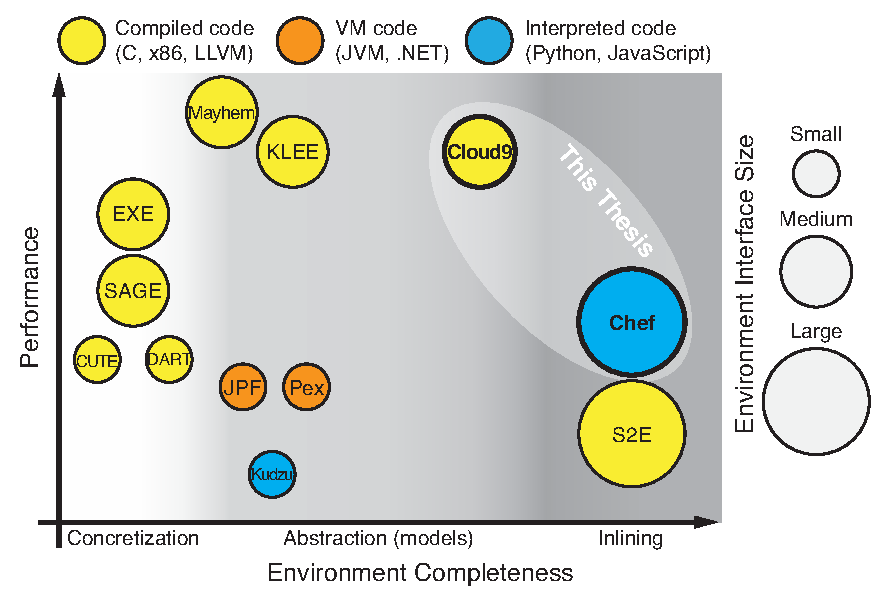
\includegraphics[width=0.8\textwidth]{figures/relwork/relwork-positioning}
  \caption{Qualitative comparison of most important symbolic execution engines with respect to the environment problem. X axis indicates completeness of symbolic environment, ranging from no symbolic support (concretization) to full environment inlining.  Y axis indicates relative performance of engines in terms of paths throughput, as deduced from each engine's evaluation numbers.}
  \label{fig:relwork:positioning}
\end{figure}

To efficiently handle real-world programs, symbolic execution engines need to minimize the time spent in the environment, while ensuring correct behavior in the program.
%
Existing approaches roughly fall into three categories, according to the degree of completeness in handling symbolic data going to the environment: (1) concretizing the calls to the environment (no symbolic support at all), (2) abstracting away the environment complexity through models, and (3) ``inlining'' the environment with the program.

Figure~\ref{fig:relwork:positioning} positions the existing work with respect to this classification, while qualitatively indicating the size of the environment interface targeted by the engine and the relative performance attained by each engine in its class.
%
In general, the less complete the environment support, the higher the engine performance is.  The engine performance is also influenced by the language level it targets: engines targeting complied code are typically faster than engines targeting high-level code.

Figure~\ref{fig:relwork:positioning} also shows that Chef and Cloud9 advance the state of the art by providing a better tradeoff between environment completeness and engine performance.
%
Cloud9 retains the performance of model-based environment handling, while providing an accurate operating system model that comes closer in completeness to an inlined approach.
%
On the other hand, Chef benefits from the completeness of inlining the environment---the language interpreter---with the interpreted program, while significantly improving performance over na\"{\i}ve symbolic execution.

In the rest of this section, we discuss in more detail each of the three environment approaches.

\subsection{Over-approximation (Concretization)}

A simple approach to simplifying the environment execution is to concretize the values that cross the program boundary~\cite{dart,godefroid:fuzz,klee,exe}.
%
For instance, when a symbolic value $\mu$ is passed as a parameter to an external function, the symbolic execution engine replaces the symbolic expression with a concrete example $m$.  This causes the execution to proceed linearly inside the environment.

For simple programs with limited interactions with their environment, this approach is sufficient.  However, for programs with stronger connections to the environment---e.g., maintaining open file descriptors---concretization may cause missed feasible paths and inconsistencies.

Consider the example of an environment call with symbolic arguments.  Concretization affects both the return value and the input arguments.
%
First, the return value is always concrete, which may lead the symbolic execution engine to miss value-dependent paths in the program, such as error handling.
%
Second, in order to maintain soundness, concretization introduces constraints in the path condition that bind the symbolic arguments to concrete examples (in our case, $pc_{new} := pc_{old} \wedge (\mu = m)$).  This, too, restricts the possible executions on the paths following the external call.
%
Avoiding the extra conditions might increase the coverage of the target program, at the expense of potentially introducing false executions.

A concrete environment may also introduce inconsistencies if it is shared among all execution paths~\cite{klee}.
%
This is commonly the case with non-concolic (``purely-symbolic'') execution, when the symbolic execution engine maintains all execution states as data structures in its address space.  Calls to the environment would then be passed on to the environment of the engine itself, potentially causing cross-talking between different execution paths.

\subsection{Abstraction (Modeling)}

An alternative approach to simplifying the environment is to replace its concrete implementation with a simpler one---a model---that captures its essential behavior~\cite{klee,mayhem,aeg}.
%
The model is smaller---often by orders of magnitude---than the original implementation, as it drops non-functional requirements, such as performance or fault-tolerance.  For example a key-value store database dependency of a web application could be replaced with a plain dictionary when symbolically executing it.

Symbolic execution engines implement models either by building them into the engine implementation (e.g., symbolic hardware models in S2E~\cite{s2eSystem}), or as guest code running together with the target program (e.g., the file system models in KLEE~\cite{klee}).

Although they are effective at reducing path explosion, models are expensive to write correctly and completely.  As a result, they tend to be employed only for simple or stable environment semantics, or when the model accuracy is less important (e.g., security testing~\cite{aeg}).

Cloud9 takes the modeling approach to the environment problem, when symbolically executing programs interacting with the operating system.  Cloud9 is the first to provide an accurate and efficient model for an operating system interface as complex as POSIX.  Key to our approach is to divide the model code into built-in core primitives and guest code, which helps keep the implementation simple, while covering much of the most common operating system abstractions.

\subsection{Inlining (Whole-system Analysis)}

Concretizing environment calls or writing models is unfeasible when the environment interface is large or maintains a complex state, strongly coupled to the program state.
%
For example, once loaded, a device driver typically can interact with the entire operating system kernel.  Concretizing all kernel calls would drastically reduce the exploration space, while modeling all kernel features would be expensive, especially for kernels with high internal churn, such as Linux.

For these cases, an approach that preserves correctness and completeness is to bundle the environment with the program and execute it symbolically as one target.
%
Full-VM symbolic execution engines provide this approach~\cite{s2e,bitBlaze}.

However, this approach reduces the effectiveness of symbolic execution on the original target program, due to the path explosion in the entire system, which may be orders of magnitude larger than the program.
%
To mitigate the path explosion, S2E introduces execution consistency models, which are principles of converting between symbolic and concrete values when crossing the program boundaries, in order to control the path explosion in the environment.

Chef takes the inlining approach to the environment problem, when symbolically executing programs written in interpreted languages.  Chef is the first system to use a language interpreter as a semantics provider for symbolic execution.


\subsection{Developer Control of Symbolic Environments}

The developer interface to a symbolic execution engine plays an important role in controlling its effectiveness and efficiency.
%
The best known sources of developer inputs are the search selection strategies and the injection of symbolic data in the system.
%
For example, KLEE runs command-line utilities with symbolic arguments defined using a special syntax, in line with the rest of the target arguments.  For instance, \codebit{ls -l --sym-arg 1 3} runs \codebit{ls} with the second argument symbolic, between 1 and 3 characters.  This syntax can be used to define symbolic arguments or symbolic files.

The developer control over the symbolic input was encapsulated in concepts such as parameterized unit tests~\cite{tillmann-puts}, which extend regular unit tests with parameters marked as symbolic inputs during symbolic execution.
%
Similarly, QuickCheck~\cite{quickcheck} allows writing input specifications in Haskell, which are used to instantiate inputs during random testing.

However, systems software is influenced by many other external factors, such as environment variables, system call failures, thread schedules, signal dispatch timing, and so on.
%
To address this problem, Cloud9's symbolic test interface gives extensive control over the behavior of its operating system model, such as per-file descriptor symbolic fault injection or per-socket symbolic control flow.


%%%%%%%%%%%%%%%%%%%%%%%%%%%%%%%%%%%%%%%%%%%%%%%%%%%%%%%%%%%%%%%%%%%%%%%%%%%%%%%%

\iffalse
\section{Path Explosion Mitigation}
\label{sec:relwork:pathexpl}

Dealing with the path explosion problem: grammar-based whitebox fuzzing (abstracting inputs), MultiSE (merging states), using symbolic execution friendly primitives (OVerify), underconstrained execution (dealing with a single module at a time).

Group heuristics by their goals and their inputs (the state information they use).

Search Heuristics in Symbolic Execution

Generational search in SAGE.

Eliminate or deprioritize the paths are are less likely to lead to the exploration goal.  Goes hand in hand with prioritization heuristics.

Replace two states meeting in the CFG with one that combines the memory locations and path conditions of the two.  Doesn't lead to improvements all the time, due to increased solver overhead [cite Trevor Hansen's study].

Compositionality means executing symbolically individual functions and storing the disjunction of path conditions as a function summary.  Can be computed incrementally, in response to program executions [cite demand-driven].

Addressing the solver bottleneck: query caches, memory models (Mayhem only models symbolic reads). Guarded sets in multiSE.

\section{Parallelizing Symbolic Execution}
\label{sec:relwork:parsymbex}

To our knowledge, we are the first to scalably parallelize symbolic execution to shared-nothing clusters.
%
\cite{parallelSymbex} described an extension to Java Pathfinder (JPF) that parallelizes symbolic execution by using parallel random searches on a static partition of the execution tree.  JPF pre-computes a set of disjoint constraints that, when used as preconditions on a worker's exploration of the execution tree, steer each worker to explore a subset of paths disjoint from all other workers.  In this approach, using constraints as preconditions imposes, at {\em every} branch in the program, a solving overhead relative to exploration without preconditions.  The complexity of these preconditions increases with the number of workers, as the preconditions need to be more selective.  Thus, per-worker solving overhead increases as more workers are added to the cluster.  This limits scalability: the largest evaluated program had 447 lines of code and did not interact with its environment.  Due to the {\em static} partitioning of the execution tree, total running time is determined by the worker with the largest subtree.  As a result, increasing the number of workers can even increase total test time instead of reducing it~\cite{parallelSymbex}.  \cnine mitigates these drawbacks.

There has been work on parallel model checking~\cite{parallelMurphi,distributed-spin,loadBalModelchecking,spin:multicore-modelchecking,modelCheckBDD}.  The SPIN model checker has been parallelized two-way for dual-core machines~\cite{parallelSPIN}. Nevertheless, there are currently no model checkers that can scale to many loosely connected computers, mainly due to the overhead of coordinating the search across multiple machines and transferring explicit states. \cnine uses an encoding of states that is compact and enables better scaling.

\fi

%%%%%%%%%%%%%%%%%%%%%%%%%%%%%%%%%%%%%%%%%%%%%%%%%%%%%%%%%%%%%%%%%%%%%%%%%%%%%%%%

\section{Symbolic Execution for High-level Languages}
\label{sec:relwork:interplang}

\subsection{Virtual Machine-based Languages: Java and C\#}

Beyond low-level system software, a significant amount of software is written in higher-level languages, offering features such as garbage collection, reflection, and built-in data structures.

Some of these languages, such as Java and C\#, are compiled to a lower-level bytecode representation and executed in a virtual machine.
%
The bytecode format is standardized and well-documented, which facilitates the development of dedicated symbolic execution engines for their runtimes.
%
For example, the Java PathFinder project~\cite{visser-jpf,jpf-symbex,jpf-testgen} provides a model checker and symbolic execution framework for Java bytecode.
%
Similarly, Pex~\cite{tillmann-pex} is a symbolic execution engine for .NET that has recently been distributed as part of the Visual Studio IDE.

The high-level environments pose additional challenges for symbolic execution related to the complexity of their data and execution model.  For example, symbolic program inputs can be both scalar and object-based.
%
Java PathFinder handles symbolic object inputs using a technique called generalized symbolic execution~\cite{generalized-symbex}, where symbolic objects are lazily initialized in response to the member accesses encountered during program execution.  Pex takes a similar approach for handling symbolic inputs in the .NET runtime.

\subsection{Dynamic Interpreted Languages}

The high-level languages that are never compiled, but source-interpreted, such as Python, JavaScript, Ruby, or Lua, are significantly more challenging for symbolic execution.
%
These languages have complex semantics that are under-specified, their features evolve rapidly from one version to another, and they rely on large built-in support libraries~\cite{dom2011,cutie-py,pythonReference}.
%
Building and maintaining a symbolic execution engine for these languages is a significant engineering effort.  As a result, the existing engines target only domain-specific subsets of their languages.

\paragraph{Supporting Symbolic Semantics}

Existing work addresses the problem of providing language semantics for symbolic execution in three major ways: by writing a symbolic interpreter for the language statements~\cite{nice}, executing the program concolically~\cite{cutie-py,jalangi}, and by requiring program cooperation~\cite{commuter}.

Writing a symbolic interpreter from scratch involves reconstructing the semantics for all the language constructs used by the target programs.  For example, the NICE-PySE~\cite{nice} symbolic execution engine, which is part of the NICE framework for testing OpenFlow applications, interprets the internal Python bytecode instructions generated by the interpreter when executing a program.  NICE-PySE is a Python application itself and uses the language reflection mechanisms to obtain, instrument and interpret the internal representation of the program.

The downside of writing a complete interpreter from scratch---including a symbolic execution engine---is that whenever a construct is not supported, the interpreter would halt.  To mitigate this, other engines take the concolic execution approach, where they run the real interpreter in concrete mode, and maintain in parallel the symbolic semantics of the language statements.  On the path segments where the symbolic semantics are not available, the execution can still make progress concretely, keeping the program state sound.  CutiePy~\cite{cutie-py} uses the tracing API of the Python interpreter to maintain the symbolic state in lockstep with the concrete execution.  The Jalangi dynamic instrumentation framework for JavaScript~\cite{jalangi} rewrites the target JavaScript program to insert statements for maintaining the symbolic state, similar to other symbolic execution engines for C programs~\cite{dart,cute,exe}.

In certain applications, symbolic execution is used to execute a model of a larger system, in the vein of model checking.  In this case, the model uses the specific API provided by the engine; the high-level language acts as a DSL, whose features are fully supported by the engine.
%
For example, the symbolic execution engine of the scalability testing tool Commuter~\cite{commuter} is entirely built in Python and offers an API for symbolically modeling operating system calls using the Python language.

In contrast to the existing techniques, Chef is the first system to use symbolic execution on an interpreter to symbolically execute a program written in the target interpreted language.  The closest work related to our approach is PokeEMU~\cite{hifi-lofi}, which uses symbolic execution on a reference CPU emulator to generate a test suite for checking the correctness of another emulator.  The generated test suite captures the semantics of the CPU instruction set, as implemented by the reference emulator.  However, the goal of PokeEMU is to check the implementation of the emulator, while in the case of Chef, we target the programs running in the interpreter.

\paragraph{Effectiveness of Symbolic Execution for Interpreted Languages}

Despite their shortcomings, the existing symbolic execution engines for interpreted languages have already shown promise for finding bugs, in areas where these languages are increasingly popular, such as web applications~\cite{saxena-kudzu,artzi-apollo, kiezun-ardilla}.

For instance, the Kudzu~\cite{saxena-kudzu} symbolic execution engine for JavaScript was used to detect code injection vulnerabilities.  The Apollo~\cite{artzi-apollo} engine targets PHP code to detect runtime and HTML errors, while Ardilla~\cite{kiezun-ardilla} discovered SQL injection and cross-site scripting vulnerabilities in PHP applications.
%
This potential is also confirmed by our findings with Chef, whose engines for Python and Lua discovered hangs and unexpected exceptions in popular packages (Section~\ref{sec:eval:bug-finding}).


\iffalse
\section{UNSORTED}

Closely related to symbolic execution is the concept of bounded model checking (BMC).  Instead of exploring individual execution paths and generate test cases, a BMC unfolds the control flow graph of the program and constructs a verification condition---a formula encompassing the behavior of the entire program with respect to a property to be checked.  Popular model checkers include CBMC~\cite{cbmc}, LLBMC~\cite{llbmc2012}, F-Soft~\cite{f-soft}, Magic~\cite{magic}, or Saturn~\cite{saturn}.

Beyond symbolic execution, there is substantial work done in the field of model checking and formal methods in general, which goes beyond the scope of this thesis.  We refer the interested reader to survey papers that cover the topic in more breadth~\cite{jhala2009software, woodcock2009formal}.

Black-box (random) fuzzing.

Unsound approaches.

Cooperative symbolic execution (where the program uses special APIs of the engine).

OVerify.
\fi

%% \paragraph{DART}

%% DART automatically extracts the environment interface of a C program using static analysis.  DART augment the classic random fuzzing with a dynamic analysis that collects. The advantage of concrete execution is that DART can fall back on concrete semantics when symbolic ones are not supported (e.g., multiplications) DART detects standard errors such as crashes, assertion violations, and hangs.  Dart extracts the static interface of a program, consisting of global variables and inputs to the program entry function.  It concretizes calls to library functions.

%% Initializing values in DART: either randomly, or NULL or malloced values (for pointer types).  Chef and Cloud9 leaves it to the symbolic test the job of creating inputs. The basic primitives are marking allocated buffers (or integers or strings) as symbolic.
%% Dealing with environment inconsistencies in DART: Not a problem, as programs are re-executed (so no cross-talking in paths).  But assume no side effects in the program.
%% Solver in DART: lp\_solve (linear constraints of integers and reals).
%% DART was applied on C benchmarks and an implementation of the SIP protocol, finding hundreds of crashes.
%% DART uses DFS, BFS, or random.

%% \paragraph{CUTE}
%% Unit testing using concolic execution, with memory graphs as inputs.  Separates memory constraints from scalar constraints and keeps pointer constraints simple to keep the decision procedure tractable and efficient.
%% CUTE uses DFS.
%% CUTE uses its own in-house solver, built on top of lp\_solve, which adds optimizations such as incrementality.
%% CUTE supports generation of structured data by either calling sequences of operations, or solving data structure invariants (repOk operations), similar to Korat~\cite{boyapati:korat}.
%% Used for testing data structures.

%% \paragraph{EXE}
%% Dedicated constraint solver STP, codesigned with EXE, optimized for reasoning about bitvectors and arrays, which accurately encode machine operations at good performance.
%% Has a flat view of memory.
%% Works by translating the C code to an instrumented format that includes checks for concrete/symbolic values, forks (UNIX forks), and checks for properties (memory errors, division by zero).
%% Introduced constraint optimization: caching, constraint independence.
%% DFS/BFS as search heuristics.
%% Found bugs in udhcpd, packet filters (BPF), pcre regexp library.

%% \paragraph{SAGE}~\cite{sage2012,godefroid:fuzz}
%% Used in production, during Windows development, found thousands of vulnerabilities.  Largest known deployment of symbolic execution in production.
%% Targeted large applications, binary-level.
%% Introduces the generational search heuristic for finding bugs more efficiently in an incomplete search.

%% \paragraph{KLEE}
%% Uses symbolic execution for testing real-world systems code (Coreutils, Hi-star kernel, Busybox).  They built a high-performance symbolic execution engine that finds bugs in highly tested code and achieves high coverage levels.
%% Compact state representation using COW.
%% Uses a high-performance SMT solver (STP), and optimizes interface to the solver (constraint caching, expression simplifications).
%% Handles the environment problem through a model of files (used by the Coreutils), and external calls into the host environment.
%% Handles C code by compiling and running LLVM.
%% Uses static heuristics to maximize coverage, plus standard strategies.
%% Command line interface for marking inputs symbolic.

%% \paragraph{AEG}~\cite{aeg}
%% Automated testing with the specific purpose of generating proofs of vulnerabilities (exploits), i.e., inputs that explicitly hijack the program control flow and get a shell.
%% Takes as input LLVM + binary, produces exploit.
%% Generated 16 exploits on 14 open-source projects.
%% Buggy path-first heuristic: When a path has a bug (unexploitable), it is likely that it'll exhibit more bugs that could be exploitable.
%% Loop exhaustion strategy: prioritize paths exploring maximum number of iterations.
%% Symbolic files: simplifies KLEE's interface.
%% Symbolic sockets: supplies fresh symbolic data.
%% Environment variables (concrete values, fully symbolic, failures).
%% Network, multithreading, formatting functions (about 70 system calls).  Not clear how sound the support is, nor what happens when a syscall is not supported.

%% \paragraph{Mayhem}~\cite{mayhem}
%% Finds 29 exploitable vulnerabilities in Linux and Windows programs.
%% System designed to handle efficiently (at the expense of completeness) large state spaces generated by large programs.  Efficient reasoning about symbolic memory (symbolic writes are concretized, symbolic reads are replaced with nested ite expressions).
%% Uses only binaries (no debug info needed).

%% \paragraph{Bitblaze}~\cite{bitBlaze}
%% Unified binary analysis platform, used mainly for malware analysis.

%% \paragraph{Java Path Finder}
%% \cite{jpf-symbex,jpf-testgen,generalized-symbex}.
%% Code that manipulates complex data structures.  Uses lazy initialization to instantiate data structures.
%% Built on top of the JVM.
%% Uses iterative deepening combined with DFS.
%% Model checking as a form of testing: since the program environment is typically way too large, model checking ends up being testing.
%% Can be used to either execute a repOk method and generate blackbox inputs, or do whitebox testing.

%% \paragraph{Pex}
%% Pex~\cite{tillmann-pex}.
%% Whitebox fuzzing for .NET.  Integrated in Visual Studio.  Found errors in a core .NET component.
%% Uses PUTs (parameterized unit tests)~\cite{tillmann-puts}.
%% Uses a ``meta-strategy'' that groups branches in equivalence classes, and then selects the lest chosen class.  Different sets of equivalence classes are chosen uniformly.
%% Constructing objects: run symbolically the object constructor.

%% \paragraph{Others}

%% Other older test input generation tools: \cite{genptrinputs}.

%% Korat~\cite{boyapati:korat}. Symstra~\cite{xie:symstra}.


%%% Local Variables: 
%%% mode: latex
%%% eval: (visual-line-mode)
%%% fill-column: 1000000
%%% TeX-master: "main"
%%% End:
